\documentclass[a4paper,10pt,notitlepage]{scrartcl}

\usepackage[T1]{fontenc}
\usepackage[english]{babel}
\usepackage[utf8x]{inputenc}
\usepackage{setspace}
\usepackage{subfig}
\usepackage{textcomp}
\usepackage{graphicx}
\usepackage{fixltx2e}
\usepackage{multirow}
\usepackage{array}
\usepackage{amssymb}
\usepackage{amsmath}
\usepackage{subfig}
\usepackage{nomencl}
\usepackage[pdfborder={0 0 0}]{hyperref}
\usepackage{natbib}
% \usepackage{makeidx}
\usepackage{nicefrac}
\usepackage{bbold}
\usepackage{gensymb}

\captionsetup{labelfont=footnotesize,textfont=footnotesize}

\newcolumntype{x}[1]{>{\begin{flushleft}$}p{#1}<{$\end{flushleft}}}
\newcolumntype{y}[1]{>{\begin{center}$}p{#1}<{$\end{center}}}
\newcolumntype{z}[1]{>{\begin{flushright}$}p{#1}<{$\end{flushright}}}
\newcolumntype{m}{>{$}l<{$}}
\newcolumntype{n}{>{$}c<{$}}
\newcolumntype{o}{>{$}r<{$}}

\newcommand{\mat}[1]{\mathbf{#1}} 

\bibliographystyle{plain}

% Title Page
\title{Scientific Visualization\\Project III}
\author{Milian Wolff}

\begin{document}
\maketitle

\begin{abstract}
In our fourth and last project for the the scientific visualization class
by Eugene Zhang we mainly investigated second order symmetric tensor fields.
Similar to the last exercise we write a JavaView based application that offers
an interface to design a tensor field using design elements. Furthermore we
extract degenerate points and visualize the separatrices.

The two other tasks in this project deepen our knowledge about vector field
topology by investigating the effects of a reverse stereographic projection.
Additionally we get acquainted with Conley indizes.

The source code of my exercise solutions can be found online under

\begin{center}\url{https://github.com/milianw/scivi}\end{center}
\end{abstract}

\begingroup
\let\clearpage\relax

\tableofcontents
\endgroup

\section{Tensor Field Design}

\begin{figure}
 \centering
 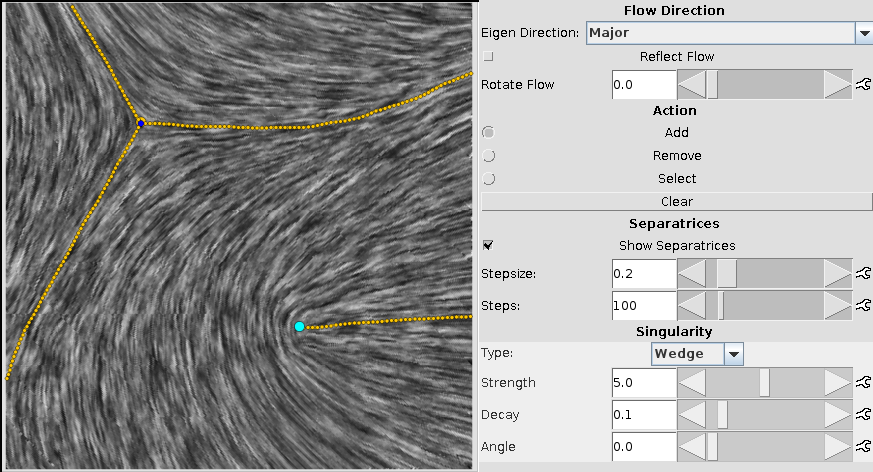
\includegraphics[scale=0.5]{img-4-2/app.png}
 \caption{Tensor Field Design Application}
 \label{fig:tfd-app}
\end{figure}

\begin{figure}
  \centering
  \subfloat[constant]{
    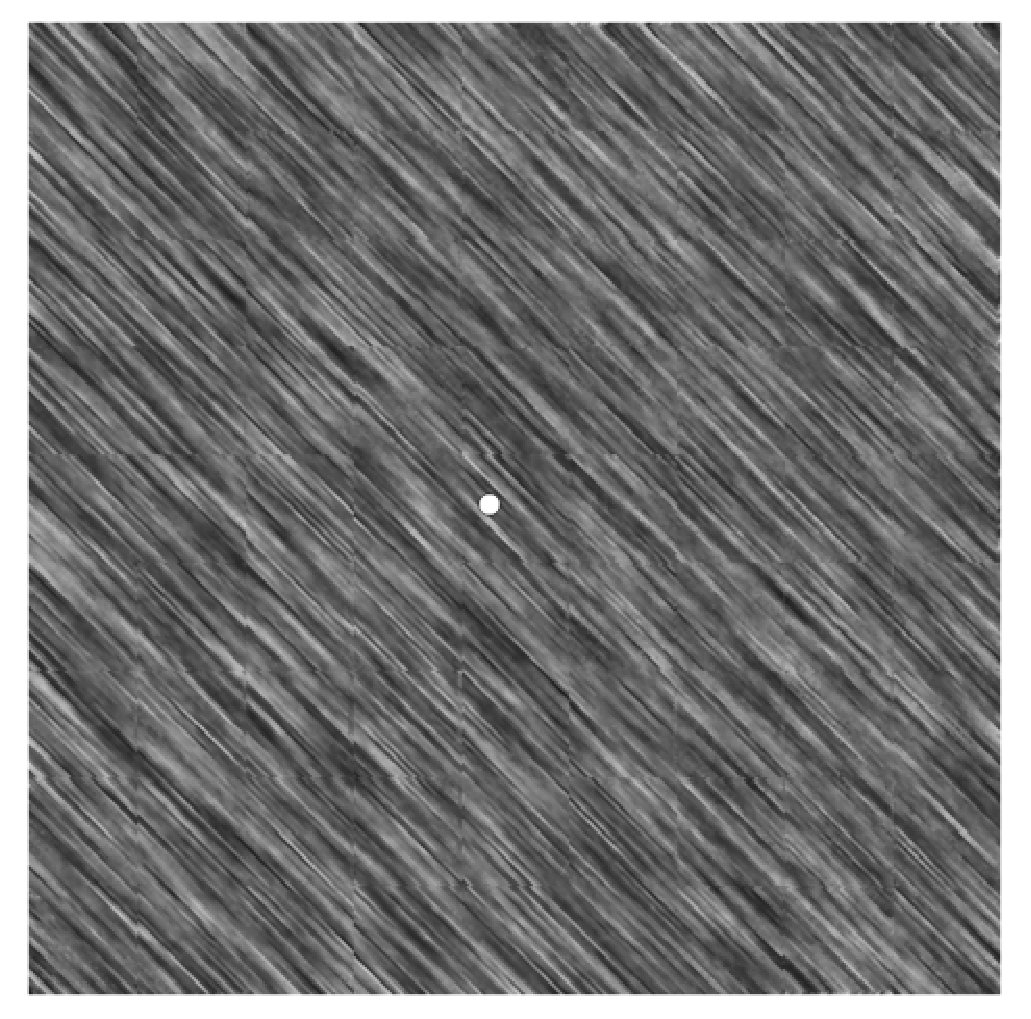
\includegraphics[width=0.3\textwidth]{img-4-2/constant.eps}}
  \subfloat[wedge]{
    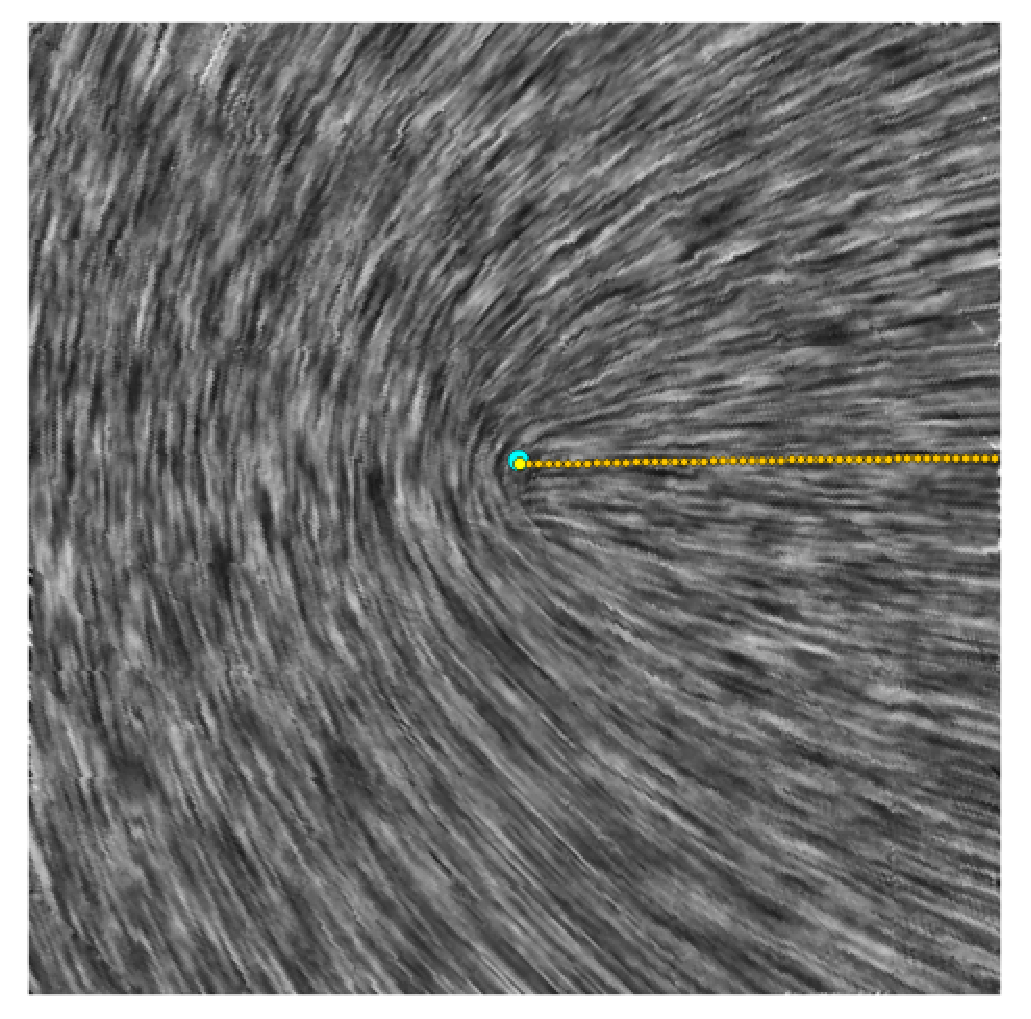
\includegraphics[width=0.3\textwidth]{img-4-2/wedge-s.eps}}
  \subfloat[trisector]{
    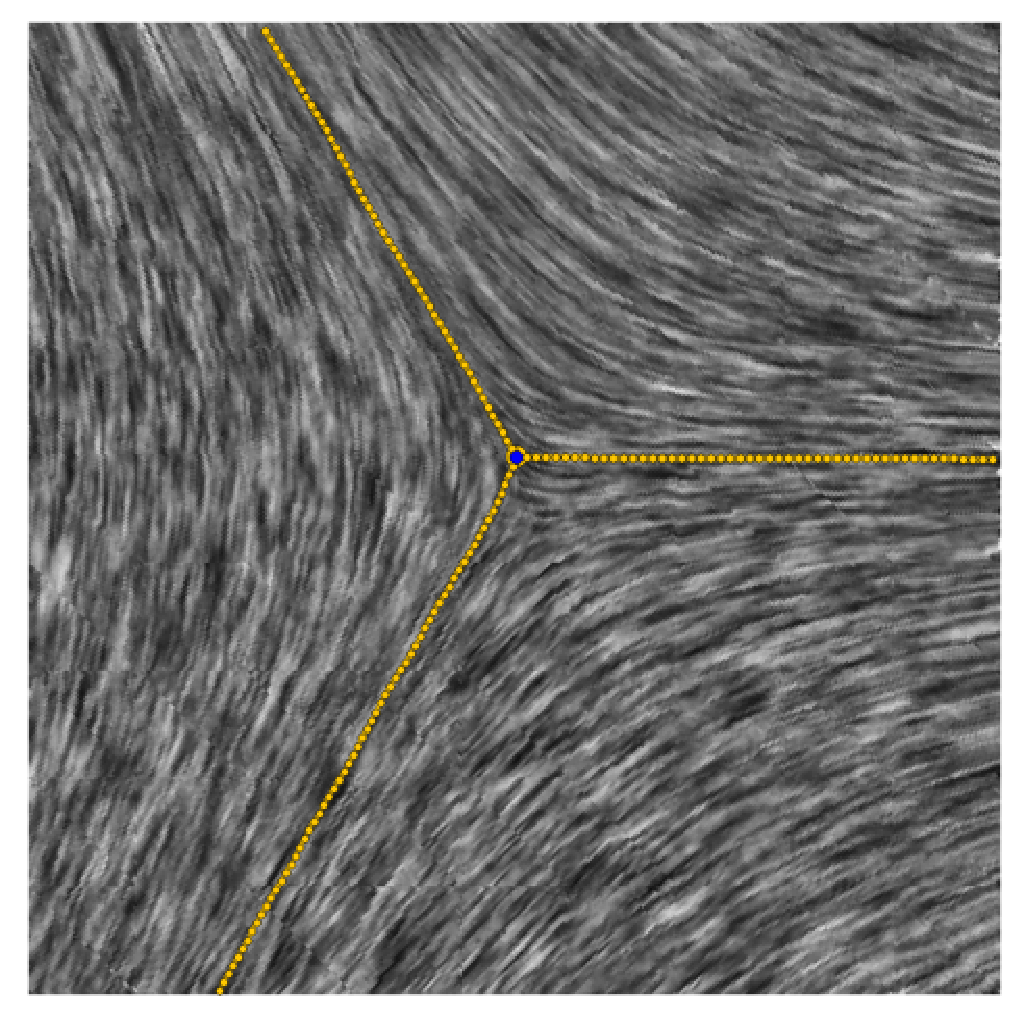
\includegraphics[width=0.3\textwidth]{img-4-2/trisector-s.eps}}
  \\
  \subfloat[node]{
    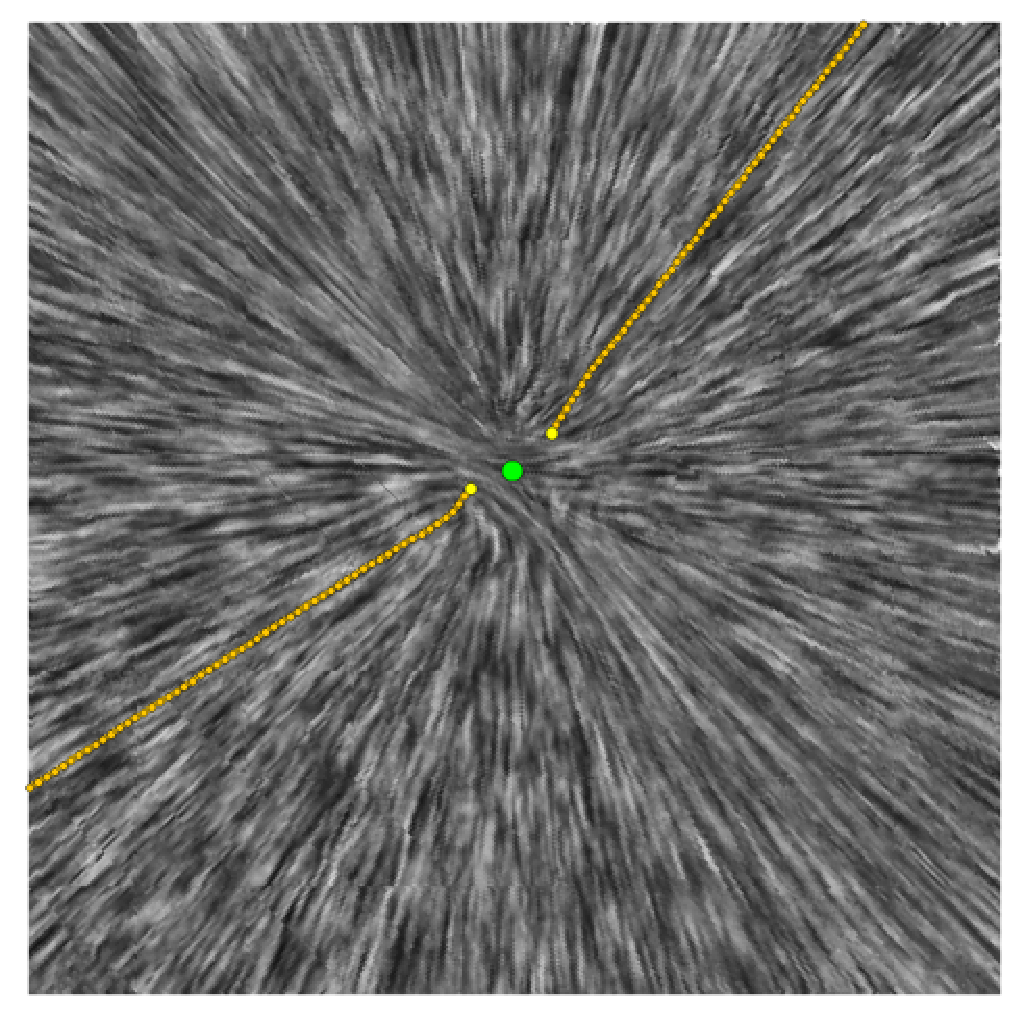
\includegraphics[width=0.3\textwidth]{img-4-2/node-s.eps}}
  \subfloat[center]{
    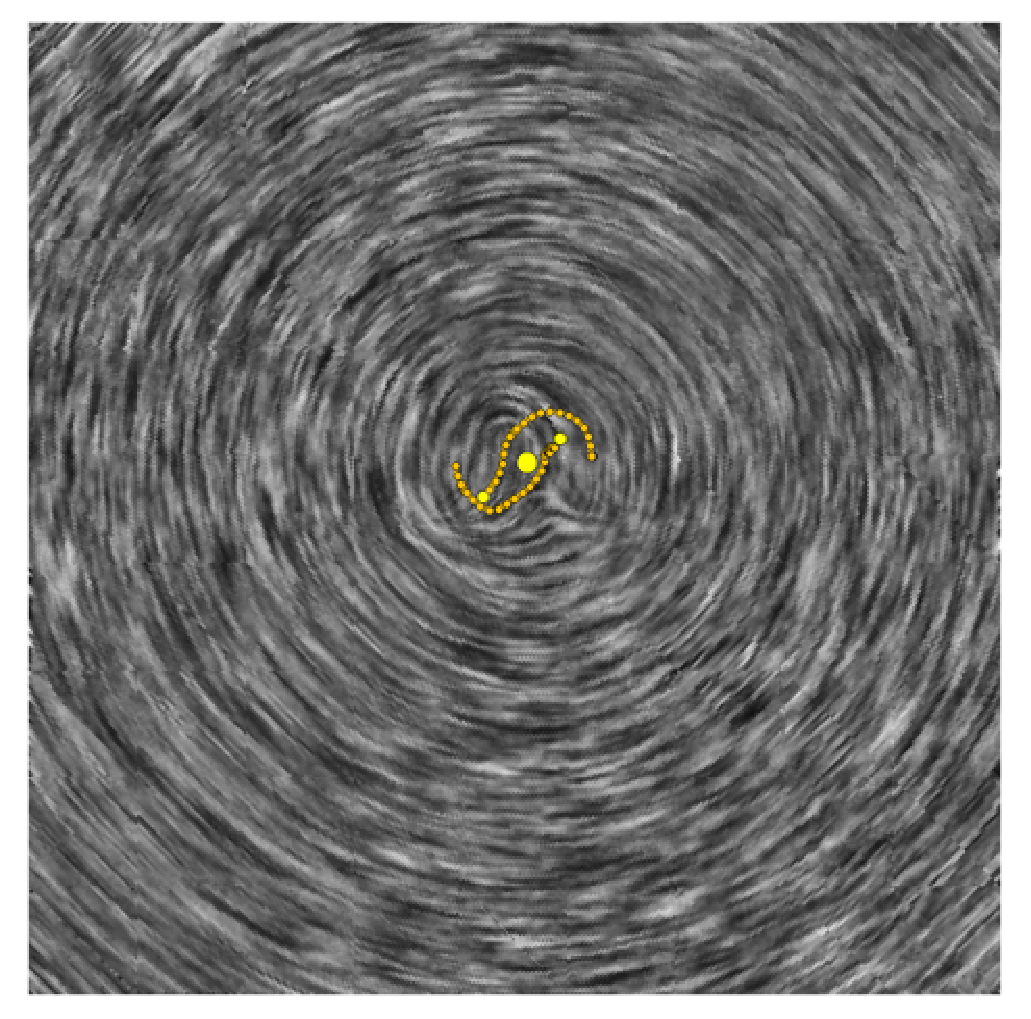
\includegraphics[width=0.3\textwidth]{img-4-2/center-s.eps}}
  \subfloat[saddle]{
    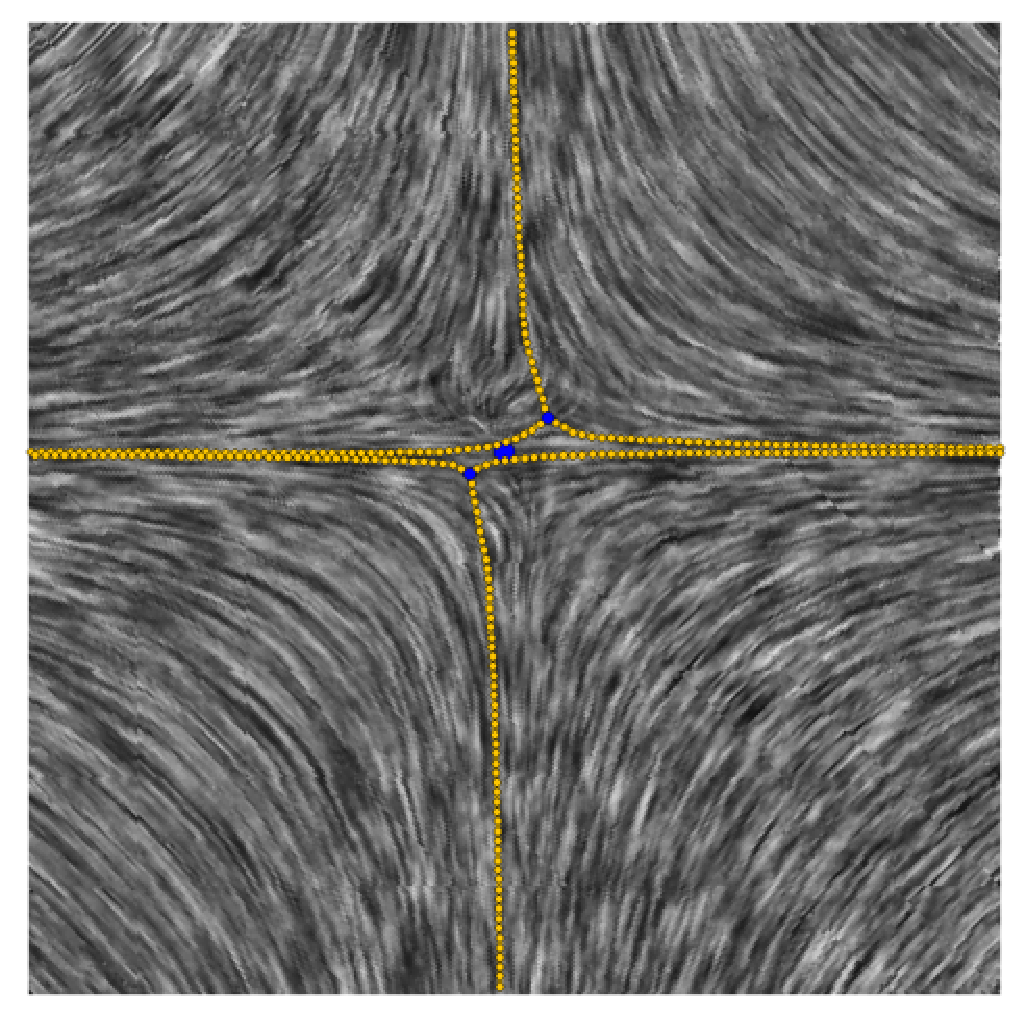
\includegraphics[width=0.3\textwidth]{img-4-2/saddle-s.eps}}
  \caption{tensor field design elements}
  \label{fig:tfd-elements}
\end{figure}

\begin{figure}
  \centering
  \subfloat[original]{
    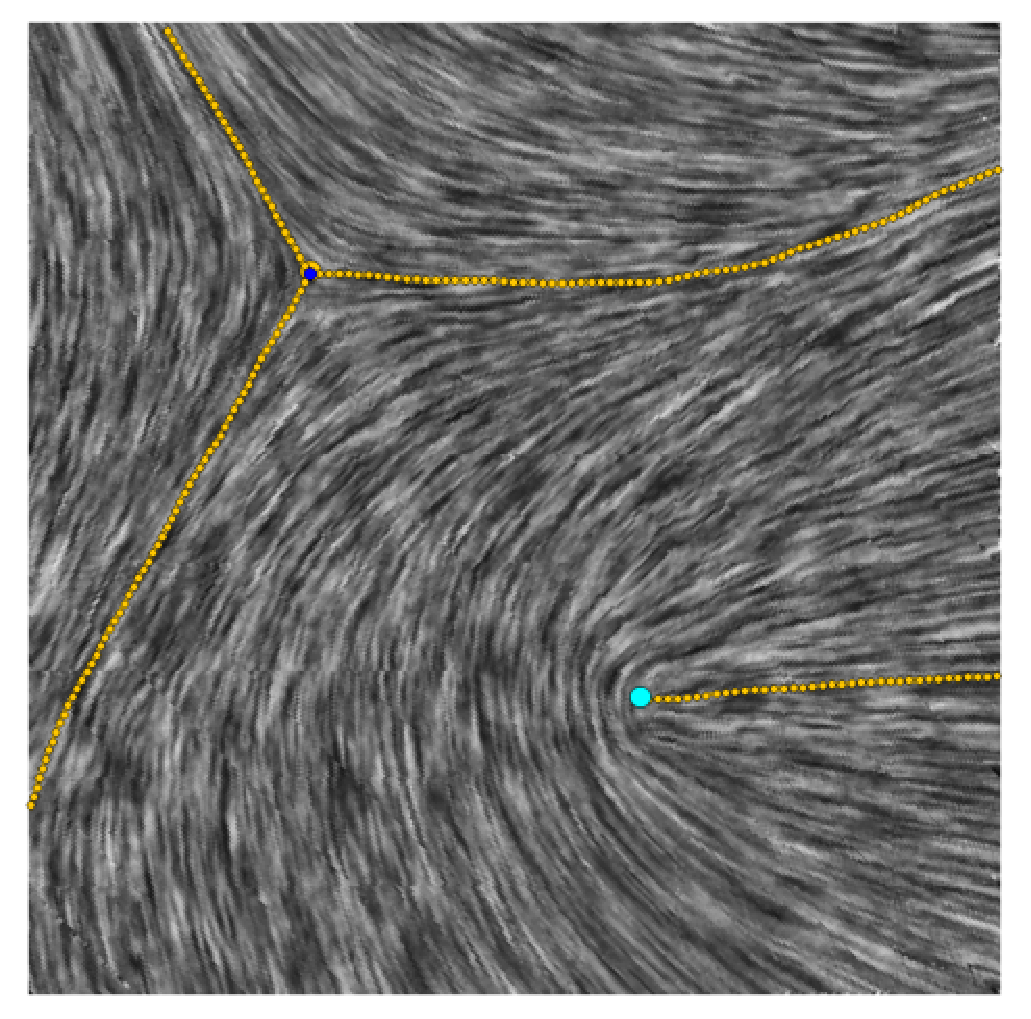
\includegraphics[width=0.3\textwidth]{img-4-2/wedge-trisector-base.eps}}
  \subfloat[$45\degree$]{
    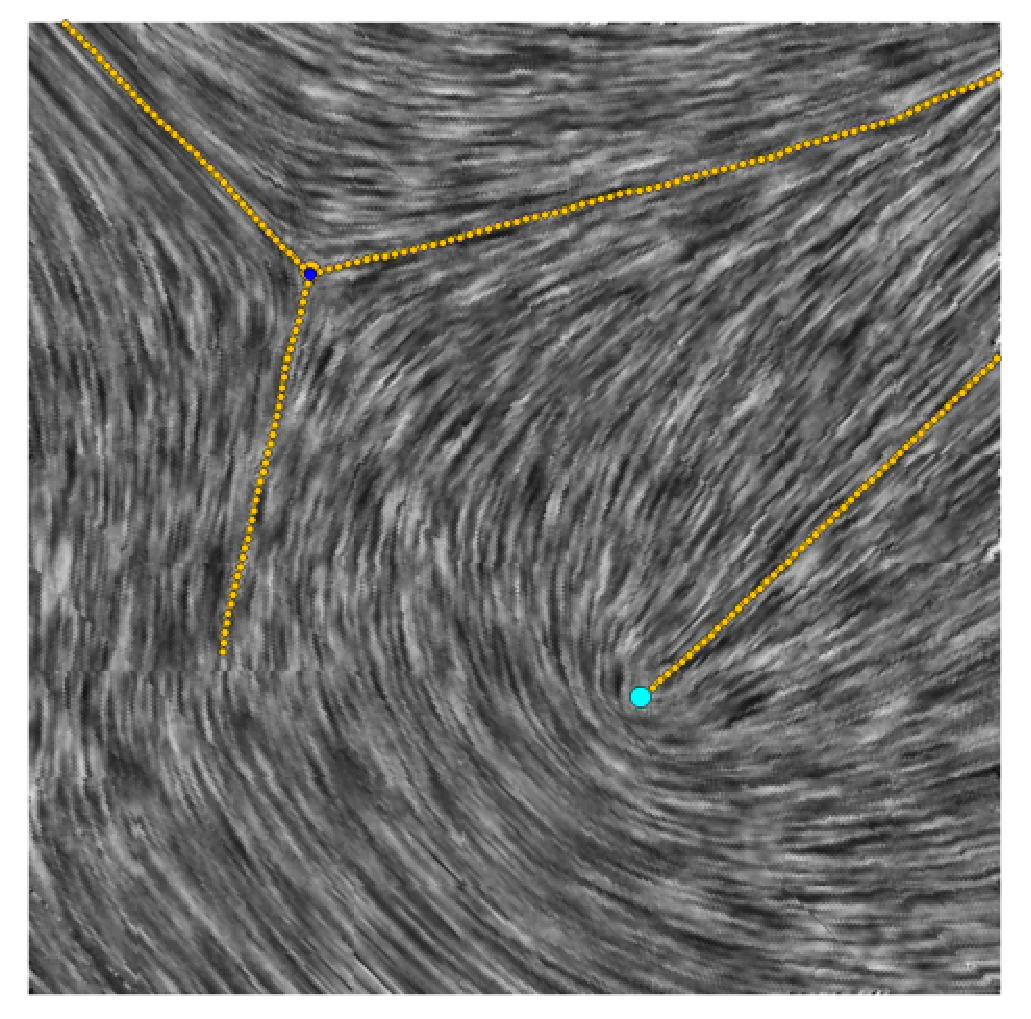
\includegraphics[width=0.3\textwidth]{img-4-2/wedge-trisector-45.eps}}
  \subfloat[$90\degree$]{
    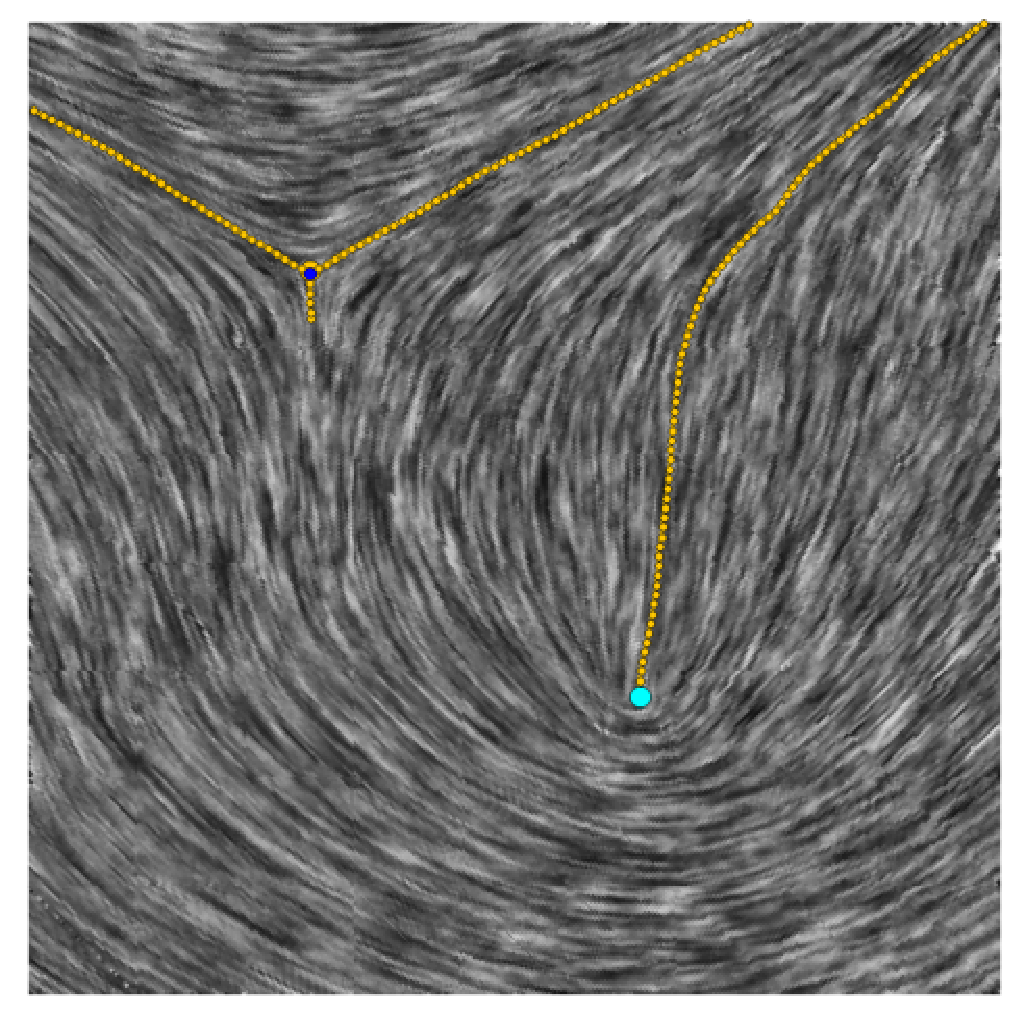
\includegraphics[width=0.3\textwidth]{img-4-2/wedge-trisector-90.eps}}
  \\
  \subfloat[$135\degree$]{
    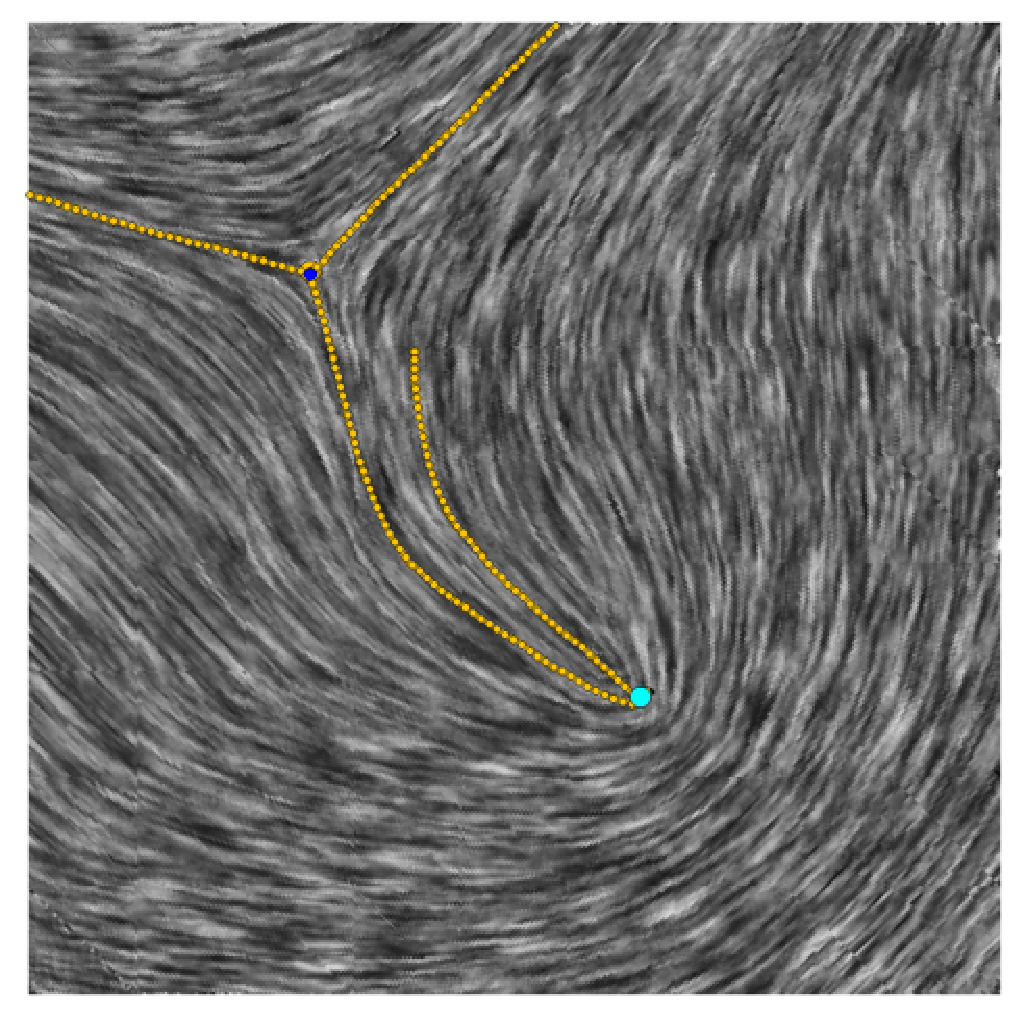
\includegraphics[width=0.3\textwidth]{img-4-2/wedge-trisector-135.eps}}
  \subfloat[$180\degree$]{
    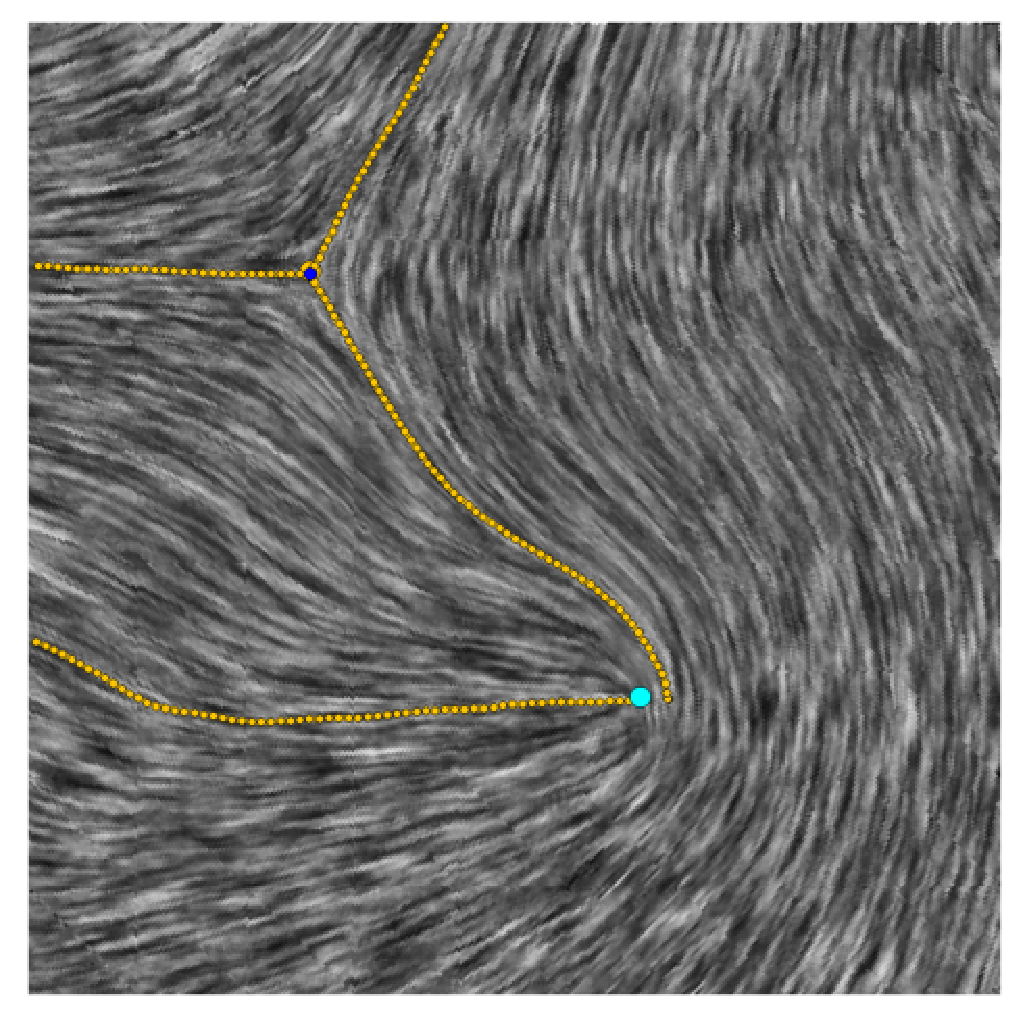
\includegraphics[width=0.3\textwidth]{img-4-2/wedge-trisector-180.eps}}
  \subfloat[$270\degree$]{
    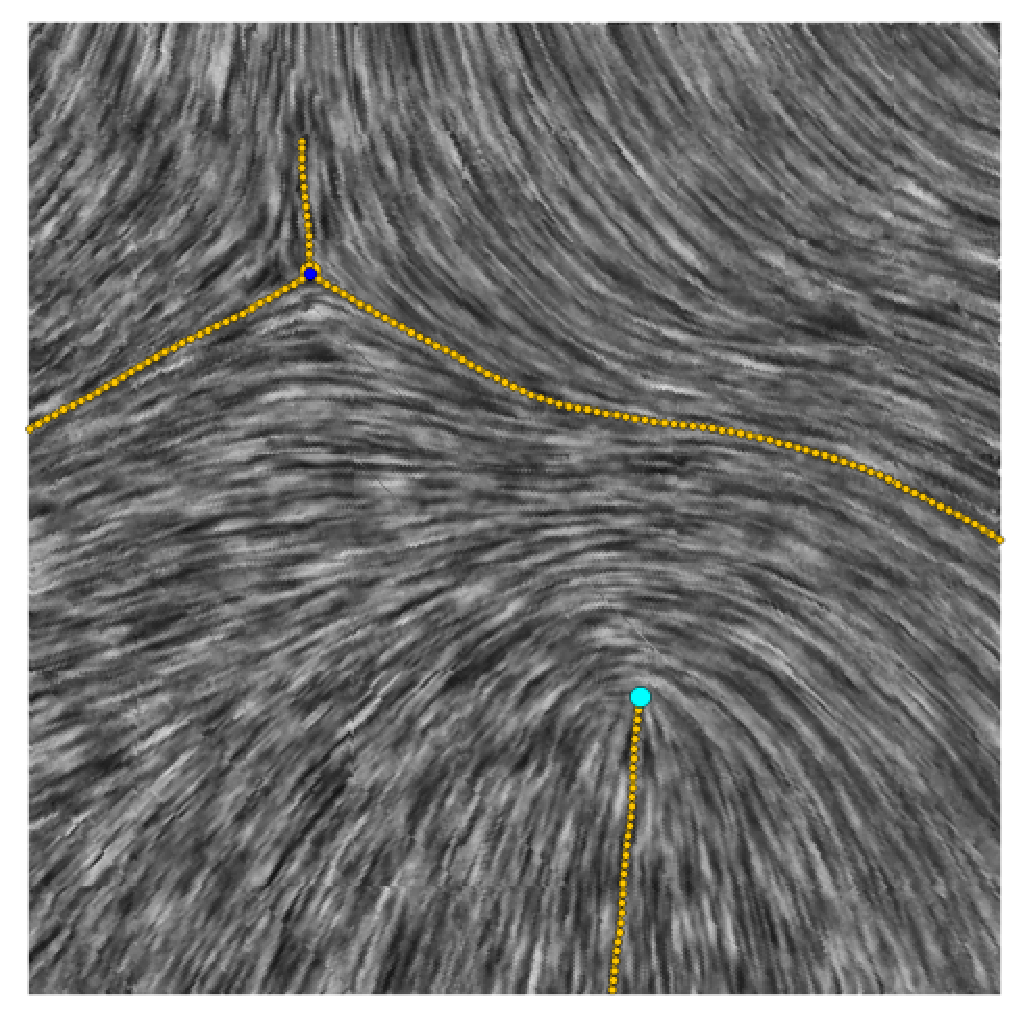
\includegraphics[width=0.3\textwidth]{img-4-2/wedge-trisector-270.eps}}
  \caption{tensor field rotation}
  \label{fig:tfd-rotation}
\end{figure}

\begin{figure}
  \centering
  \subfloat[original]{
    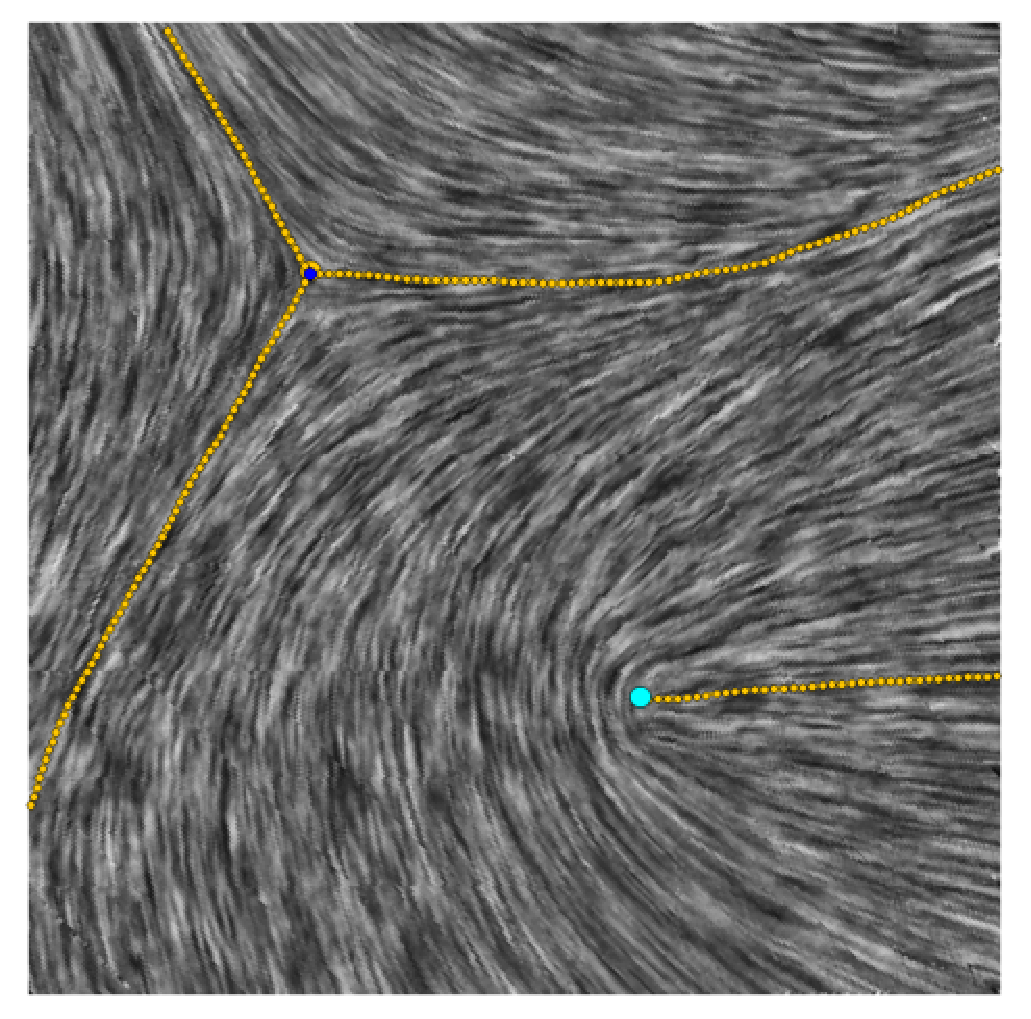
\includegraphics[width=0.4\textwidth]{img-4-2/wedge-trisector-base.eps}}
  \subfloat[reflected]{
    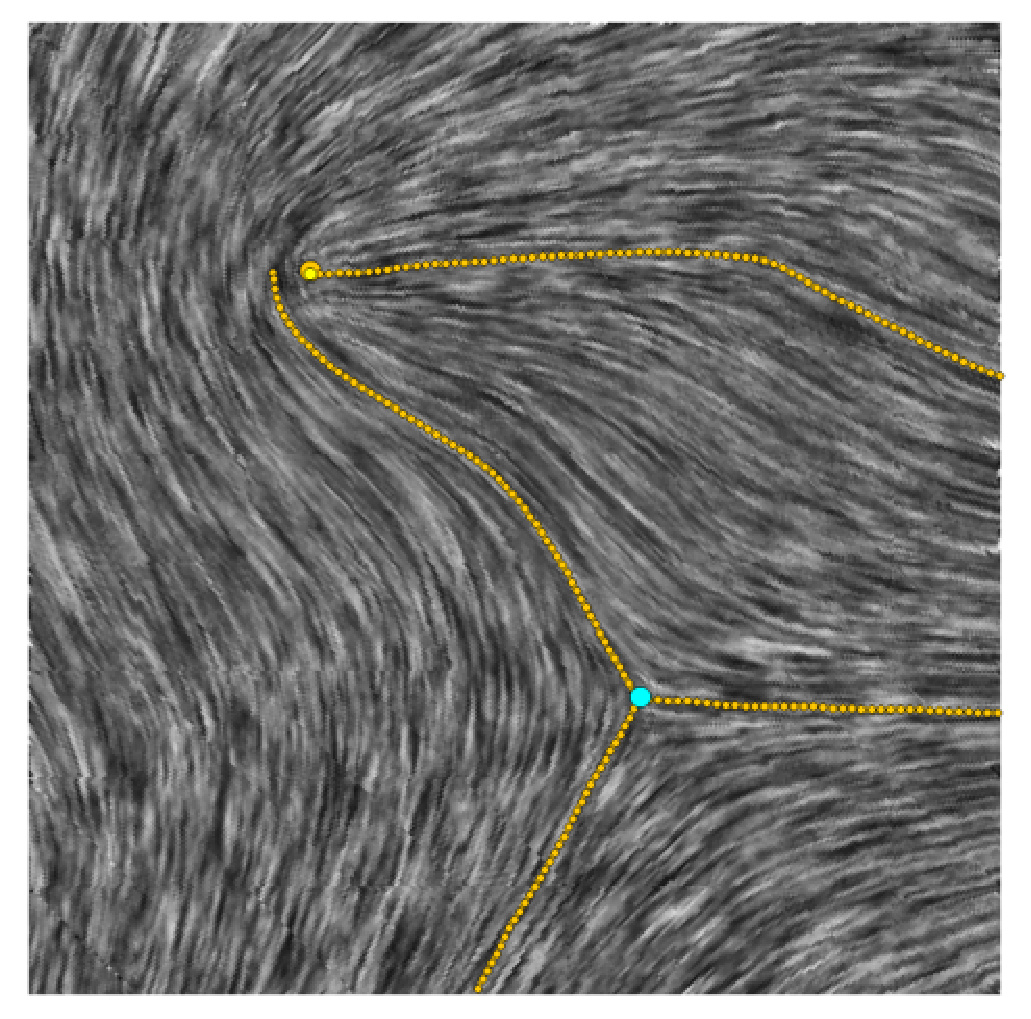
\includegraphics[width=0.4\textwidth]{img-4-2/wedge-trisector-reflect.eps}
  }
  \caption{tensor field reflection}
  \label{fig:tfd-reflection}
\end{figure}

\begin{figure}
  \centering
  \subfloat[major]{
    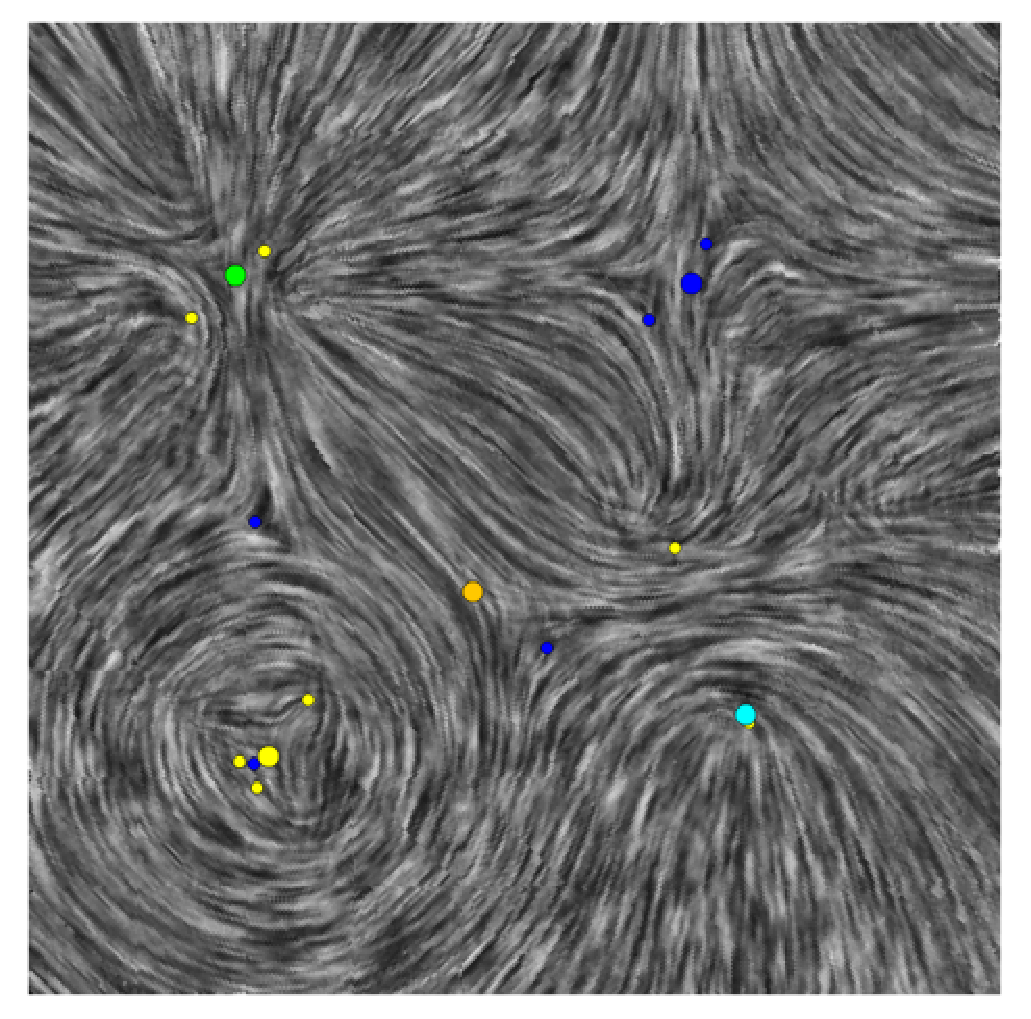
\includegraphics[width=0.4\textwidth]{img-4-2/major.eps}
    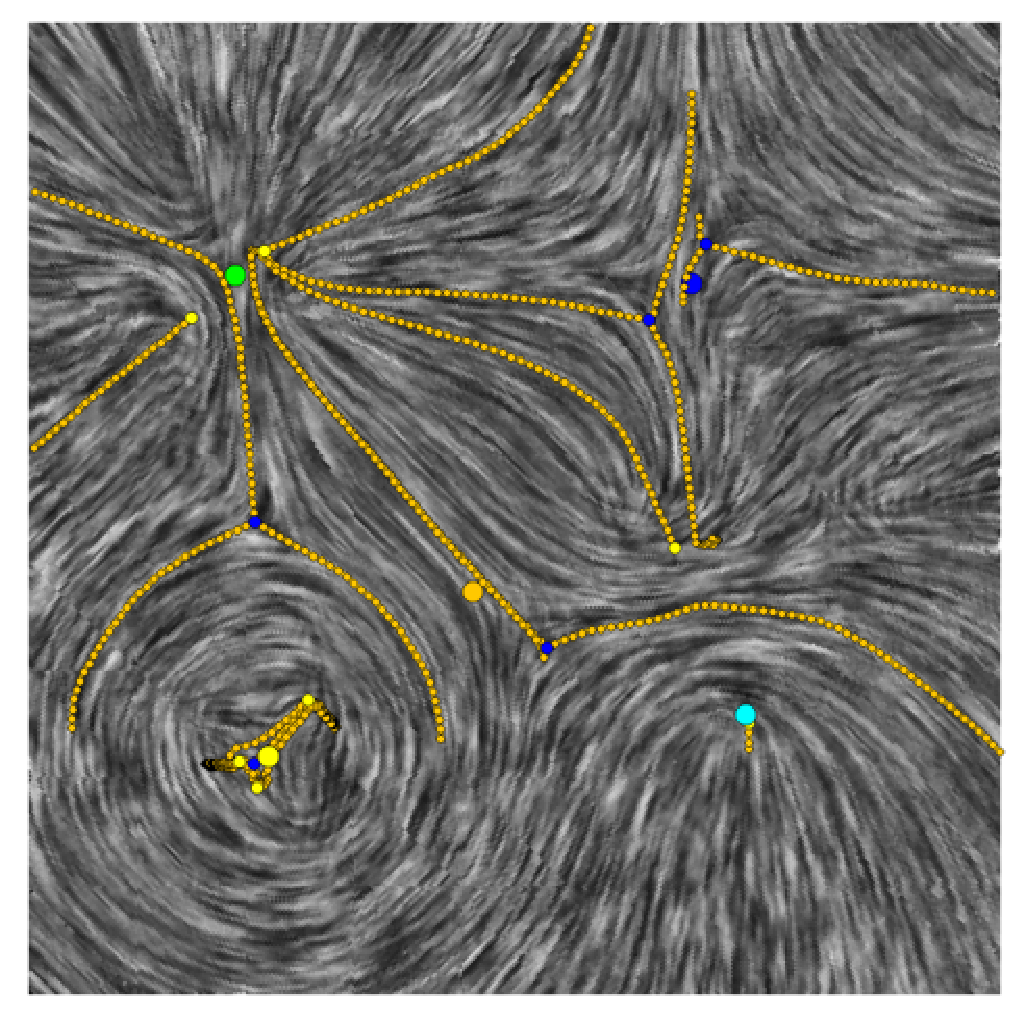
\includegraphics[width=0.4\textwidth]{img-4-2/major-s.eps}
  }
  \\
  \subfloat[minor]{
    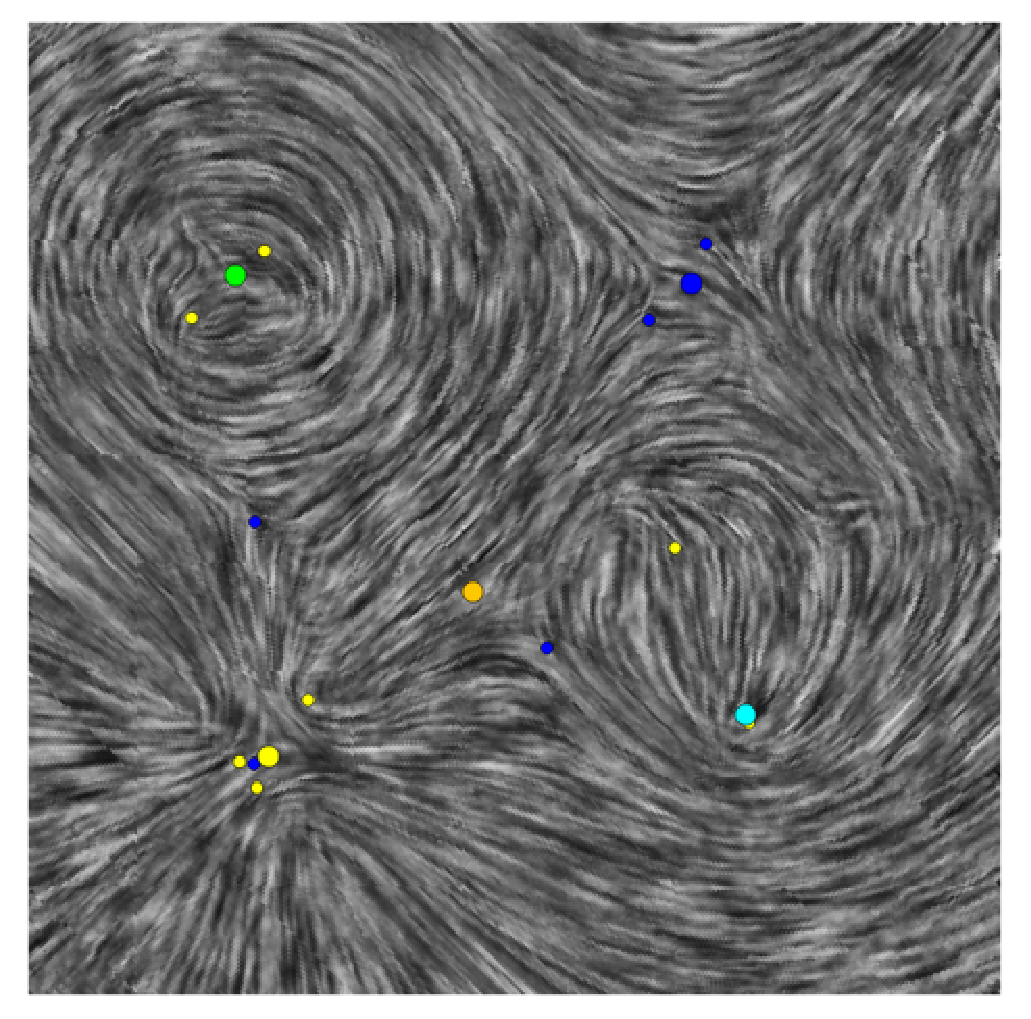
\includegraphics[width=0.4\textwidth]{img-4-2/minor.eps}
    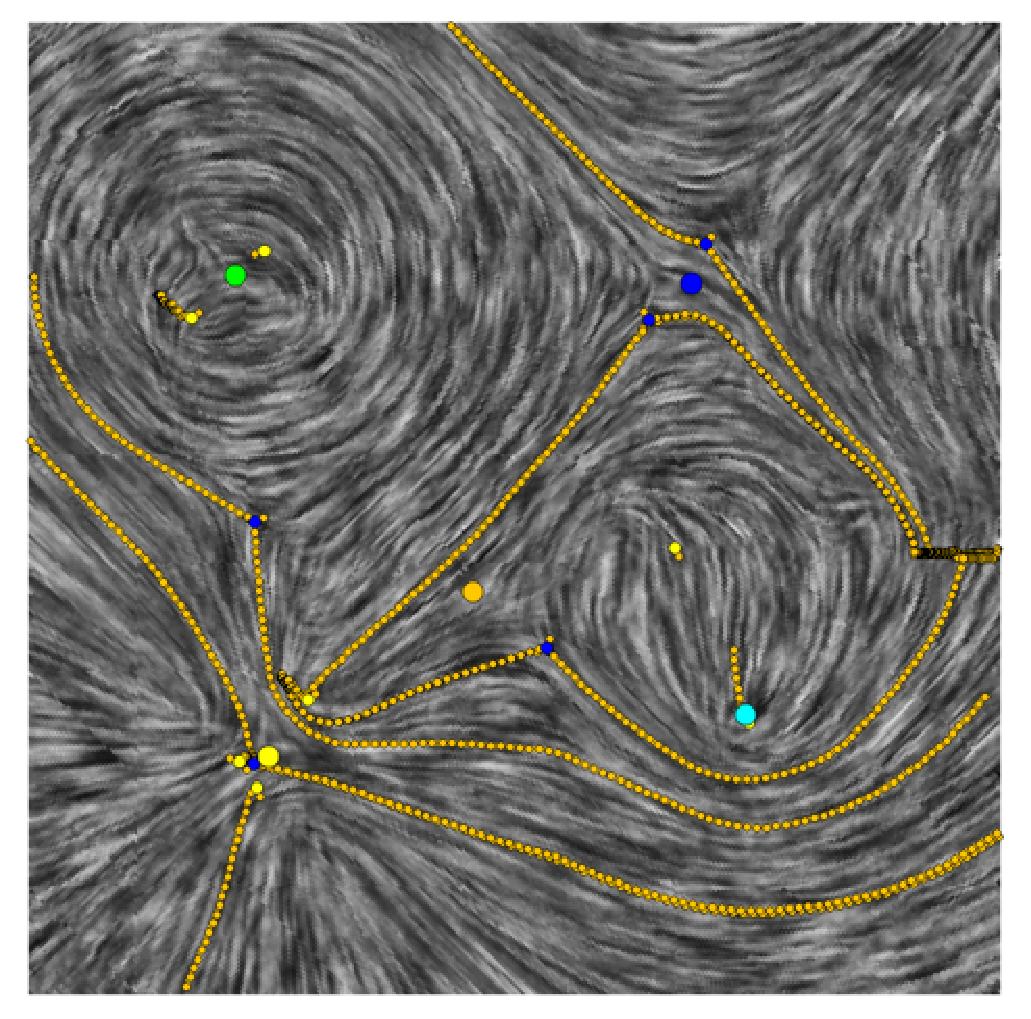
\includegraphics[width=0.4\textwidth]{img-4-2/minor-s.eps}
  }
  \caption{minor and major eigenvector fields}
  \label{fig:tfd-majorminor}
\end{figure}

\end{document}

% kate: replace-tabs on;